\section{Waarover en Hoe Denken Economen?}

Economie heeft een \term{materieel voorwerp} (\textit{`waarover gaat economie?'}) en een \term{formeel voorwerp} (\textit{`wat is de invalshoek van de econoom?'}). Deze worden respectievelijk \term{economy} en \term{economics} genoemd. Economics is ...
\begin{leftbar}
\textit{`... the science which studies human behavior as a relationship between ends and scarce means which have alternative uses' (Robbins, 1932)}\\
\par\textit{`... the study of how people interact with each other, and with the natural environment, in producing livelihoods' (The Economy-The Core Project)}
\end{leftbar}

\subsection{Bruto Binnenlands Product}\label{sec:h1bbp}

E\'en van de maatstaven die men in de economie gebruikt is het \entrystyled{bbp}{Bruto Binnenlands Product (BBP)} : \textit{de som van de gedurende \'e\'en jaar door alle binnenlandse productie-eenheden toegevoegde waarden}.
\par Dit kan men uiteraard benaderen aan de hand van de productie, via de \entry{toegevoegde waarde} (de waarde van de productie - de \textit{output} - minus de waarde van \textit{lopende inputs} of \entry{intermediaire goederen} - de grond- en hulpstoffen).
\par Deze toegevoegde waarde komt overeen met het inkomen van de bezitters van de productiefactoren (d.i., van arbeid en kapitaal). Een inkomen dat vervolgens wordt besteed aan goederen en diensten (consumerende gezinnen, overheidsconsumptie, investeringen en export minus de import). Men kan het BBP dus, naast de toegevoegde waarde, ook benaderen aan de hand van het inkomen of de bestedingen.\\

\par De evolutie van (de ordegrootte van) het BBP kan worden voorgesteld door een \entry{tijdsreeks} (door de eeuwen heen) of met \entry{doorsnedegegevens} (per regio). Tabel \ref{tab:h1bbp} is hier een voorbeeld van. 
\par Om productie doorheen de tijd vergelijkbaar te maken moet men de prijsverandering doorheen de tijd (door inflatie) in rekening brengen. Het resultaat noemt men \entrystyled{reele groei}{re\"ele groei} (de kwantiteiten veranderen). Houdt men geen rekening met prijsveranderingen dan heeft men het over \entry{nominale groei} (zowel de kwantiteit als de prijs verandert). De re\"ele groei is dan ook gelijk aan de nominale groei waarvan de inflatie wordt afgetrokken. En het is die groei die een effect heeft op de tijdsreeksen (in tabel \ref{tab:h1bbp} zijn de producties gewaardeerd tegen de prijzen van 1990).
\par Hoe maakt men de doorsnedegegevens nu vergelijkbaar? Vergelijken aan de hand van de wisselkoers (\textit{`hoeveel Amerikaanse dollars is een Chinese renmibi waard?'}) is geen goede methode ; producten hebben verschillende prijzen in verschillende landen\footnote{Een fles parfum zal in Californi\"e hoogstwaarschijnlijk m\'e\'er kosten dan in China.}. Nee, men gaat eerder vergelijken door de prijzen van producten uit het ene land te vergelijken op basis van de prijzen in het andere. Men spreekt van \entry{koopkrachtpariteit (KKP)} (in tabel \ref{tab:h1bbp} worden koopkrachtpariteitsdollars - `\term{PPP-dollars}' - gebruikt). De dollar heeft dan overal dezelfde koopkracht. Zo kan men vergelijken in de ruimte.\\

\begin{table}[H]
\small\centering\captionsetup{justification=centering,margin=2cm}
\begin{tabular}{l | c | c | c | c | c | c | c | c}
\textbf{Jaar} & \textbf{1} & \textbf{1000} & \textbf{1500} & \textbf{1820} & \textbf{1913} & \textbf{1950} & \textbf{1973} & \textbf{2015} \\
\textbf{Wereld BBP (miljarden 1990-PPP-dollars)} & 105 & 120 & 248 & 695 & 2733 & 5337 & 16022 & 59205 \\
\textbf{Wereldbevolking (miljoenen)} & 226 & 267 & 438 & 1042 & 1791 & 2526 & 3916 & 7347 \\
\textbf{BBP per hoofd in de wereld} & 467 & 450 & 567 & 667 & 1526 & 2113 & 4091 & 8059 \\
\textbf{Maandelijks BBP per hoofd in de wereld} & 39 & 38 & 47 & 56 & 127 & 176 & 341 & 672 \\
\textbf{Maandelijks BBP per hoofd in Belgi\"e} & - & - & 73 & 110 & 352 & 455 & 1014 & 1992 \\
\textbf{Maandelijks BBP per hoofd in W-Europa} & 48 & 36 & 64 & 100 & 288 & 382 & 951 & 1854 \\
\textbf{Maandelijks BBP per hoofd in de V.S.} & - & - & 33 & 105 & 442 & 797 & 1391 & 2712 \\
\textbf{Maandelijks BBP per hoofd in China} & 38 & 38 & 50 & 50 & 46 & 37 & 70 & 593 \\
\textbf{Maandelijks BBP per hoofd in Afrika} & 39 & 36 & 35 & 35 & 53 & 74 & 118 & 170 \\
\textbf{Wereldexport (miljarden 1990-PPP-dollars)} & - & - & 0 & 6 & 212 & 296 & 1691 & 14906 \\
\end{tabular}
\caption{Het BBP voor een aantal regio's doorheen de tijd (bronnen : OECD; IMF; World Development Indicators; UNCTAD; Maddison A. (2001, 2003, 2010); eigen berekeningen)}
\label{tab:h1bbp}
\end{table}

\par Figuur \ref{fig:h1growth} geeft het BPP van verscheidene regio's op \entrystyled{logaritme}{logaritmische schaal} weer\footnote{Meer info over de logaritme vind u in de appendix.}. Het is duidelijk dat China, voorheen een armer land, snel de rijkere landen inhaalt. Men noemt dit economische \entry{convergentie}. Het omgekeerde (wat voor Afrika het geval is) noemt men economische \entry{divergentie}. \\

%\begin{figure}[H]
%\small\centering\captionsetup{justification=centering,margin=2cm}
%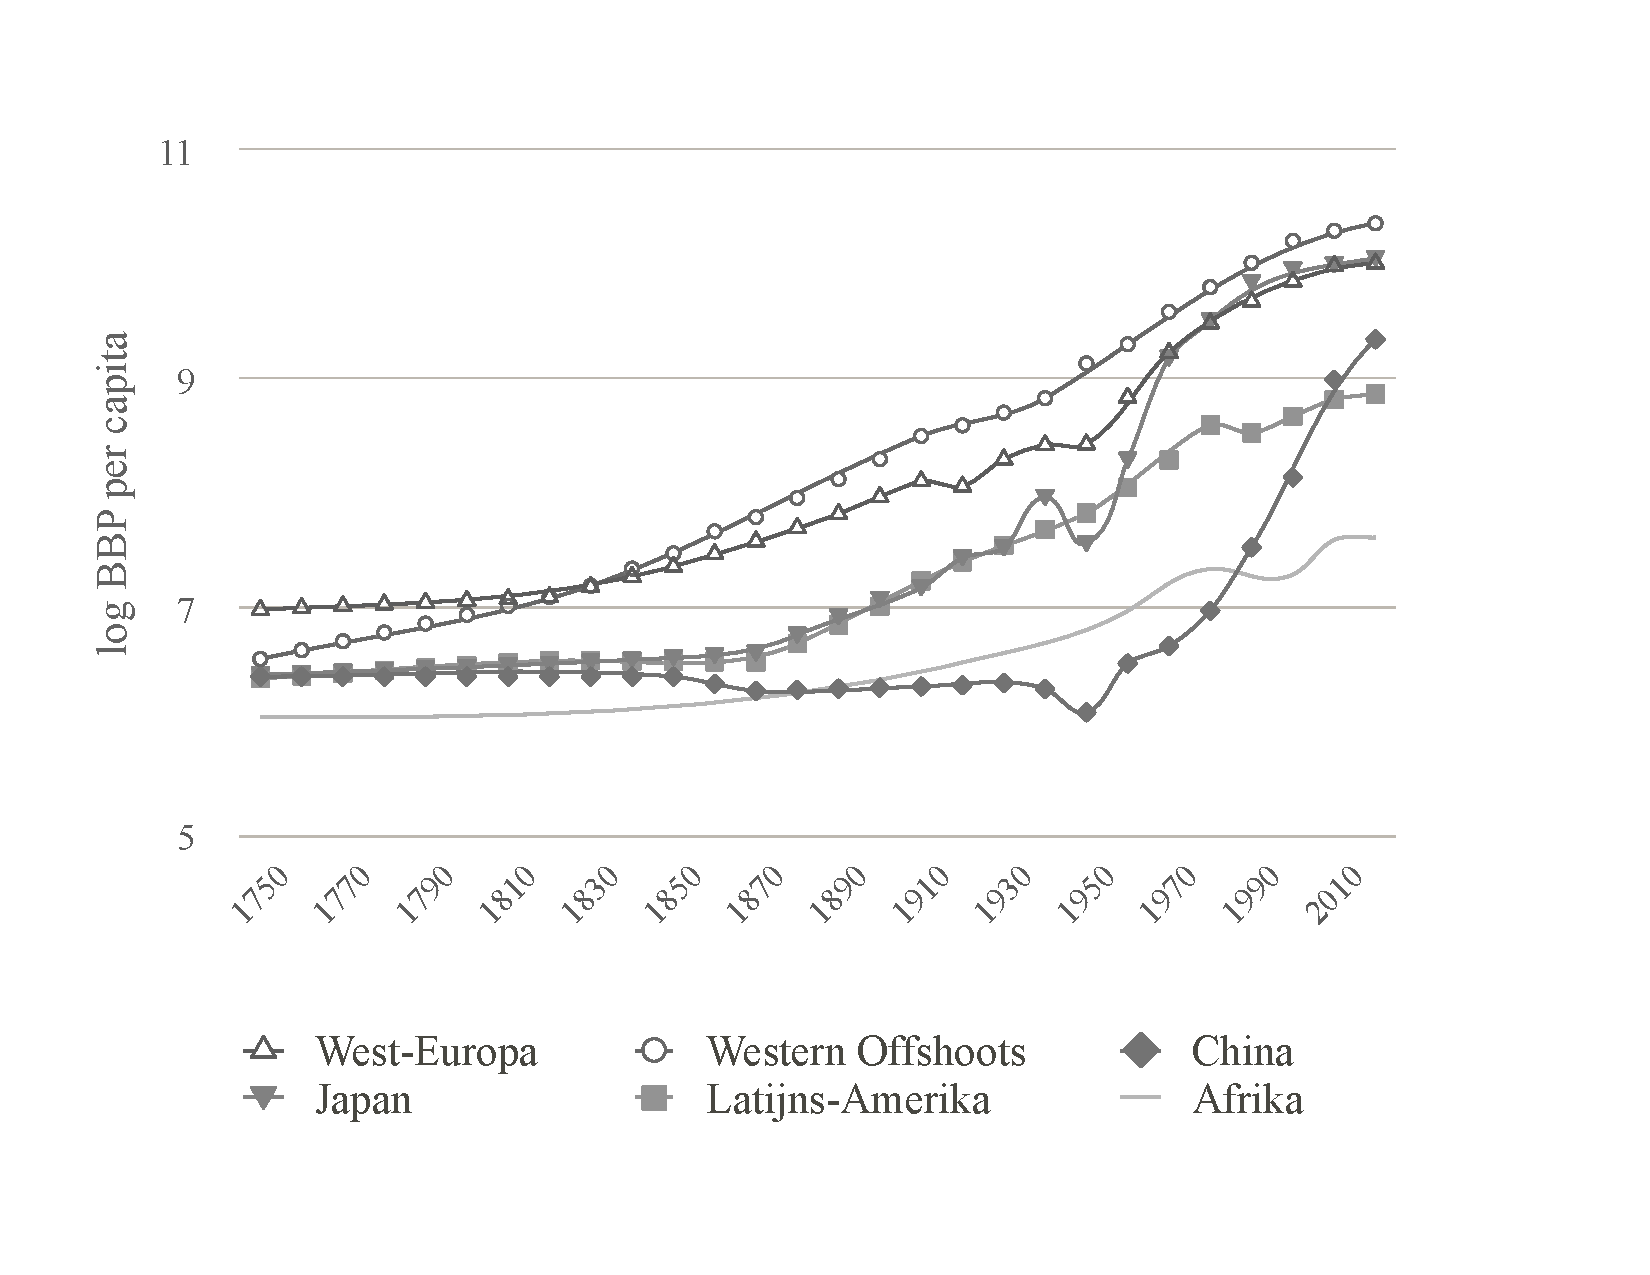
\includegraphics[width=\textwidth]{Afbeeldingen/H1-EconGroeiPDF.pdf}
%\caption{Het BBP per capita van verscheidene regio's sinds 1750, op logaritmische schaal}
%\label{fig:h1growth}
%\end{figure}

\begin{figure}[H]
\small\centering\captionsetup{justification=centering,margin=2cm}
\begin{tikzpicture}
\begin{axis}[axis lines=left,axis line style=gray,/pgf/number format/.cd, use comma, 1000 sep={}, width=0.8\linewidth, legend cell align=left, legend pos=north west,legend style={draw=none},ylabel={log($BBP$) per capita}]
\addplot[gray, mark=x, mark options = {draw=blue,fill=blue}] table [x=Jaar, y=West-Europa, col sep=comma] {Data/H1-EconGroei.csv};
\addplot[gray, mark=+, mark options = {draw=blue,fill=blue}]  table [x=Jaar, y={Western Offshoots}, col sep=comma] {Data/H1-EconGroei.csv};
\addplot[gray, mark=star, mark options = {draw=blue,fill=blue}]  table [x=Jaar, y=China, col sep=comma] {Data/H1-EconGroei.csv};
\addplot[gray, mark=triangle, mark options = {draw=blue,fill=blue}]  table [x=Jaar, y=Japan, col sep=comma] {Data/H1-EconGroei.csv};
\addplot[gray, mark=o, mark options = {draw=blue,fill=blue}]  table [x=Jaar, y=Latijns-Amerika, col sep=comma] {Data/H1-EconGroei.csv};
\addplot[gray, mark=|, mark options = {draw=blue,fill=blue}]  table [x=Jaar, y=Afrika, col sep=comma] {Data/H1-EconGroei.csv};
\addlegendentry{West-Europa}
\addlegendentry{Western Offshoots}
\addlegendentry{China}
\addlegendentry{Japan}
\addlegendentry{Latijns-Amerika}
\addlegendentry{Afrika}
\end{axis}
\end{tikzpicture}
\caption{Het BBP per capita van verscheidene regio's sinds 1750, op logaritmische schaal}
\label{fig:h1growth}
\end{figure}

\par Merk wel op dat mensen nu anders consumeren en produceren dan voorheen. In 1853 gaf men veel meer uit aan voedsel. Veel minder (80\% minder) mensen zijn ook tewerkgesteld in de landbouw. Dit moet in rekening gebracht worden bij het interpreteren van voorgaande cijfers.

\subsection{Productiviteit}\label{sec:h1prod}

Het \entrystyled{bbp}{Bruto Binnenlands Product (BBP)} kan als volgt ontleed worden :
$$\frac{\text{bbp}}{\text{bevolking}}=\frac{\text{bbp}}{\text{\#uren}}\cdot\frac{\text{\#uren}}{\text{\#werkenden}}\cdot\frac{\text{\#werkenden}}{\text{beroepsbevolking}}\cdot\frac{\text{beroepsbevolking}}{\text{\#15-65-jarigen}}\cdot\frac{\text{\#15-65-jarigen}}{\text{bevolking}}$$
De eerste factor (het BBP per aantal uren) is de \entry{arbeidsproductiviteit}. Het is de enige factor die geen bovengrens heeft, en die dus verantwoordelijk is voor onze huidige rijkdom. Hij stijgt door investeringen in machines en door technologische vooruitgang.
\par\noindent De tweede factor is het aantal gewerkte uren, de \entry{arbeidsduur}, wat doorheen de jaren significant verminderd is (van zo'n 57 tot zo'n 30 uren per week).
\par\noindent De derde factor is de \entry{activiteitsgraad} of \entry{participatiegraad} - het zijn diegenen die \textit{kunnen} werken, zij die werk gevonden hebben. Het complement hiervan (1 minus de participatiegraad) is de \entry{werkloosheidsgraad}. 
\par\noindent De voorlaatste factor is het aantal mensen die \textit{willen} werken, die hun arbeid aanbieden op de arbeidsmarkt. 
\par\noindent De laatste factor is het aandeel van 15-65-jarigen, die omwille van de \entry{vergrijzing} daalt. 
\par\noindent De verhouding tussen het aantal werkenden ($\text{\#werkenden}$) en de bevolking in de beroepsactieve leeftijd ($\text{\#15-16-jarigen}$) noemt men de \entry{werkgelegenheidsgraad}.

\subsection{Specialisatie \& Ruil}

Wat men verbruikt of gebruikt maken we niet allemaal zelf. We specialiseren en ruilen. Er is dus \entry{arbeidsverdeling}.
\par\noindent Allereerst is er \textbf{horizontale -}\index{horizontale arbeidsverdeling} of \term{sociale arbeidsverdeling}. Er wordt verdeeld \textit{per product}. Zo heb je juristen, software-ontwikkelaars, slagers, bakkers, ... 
\par\noindent Verder kan men ook de productiefase onderverdelen. Dit is \textbf{verticale -}\index{verticale arbeidsverdeling} of \term{technische arbeidsverdeling}. Dat zie je bij de productie van wagens (design, banden, carrosserie).
\par En op internationaal niveau is er \term{internationale arbeidsverdeling} ; we importeren en exporteren via \entry{internationale handel}. Zo heb je internationale \term{supply chains}, zoals bij de fabricatie van GSM's.\\

\par Arbeidsverdeling vraagt \textit{co\"ordinatie}. Men onderscheidt drie ideaaltypes : 
\begin{itemize}
\item \term{Traditionele systemen} : co\"ordinatie gebeurt op basis van sociale normen (van vader op zoon, tussen man en vrouw, ...). Dergelijke systemen zijn statisch. Ze zijn niet bestand tegen externe schokken (zoals contacten met de buitenwereld en nieuwe technologie\"en).
\item \term{Bevelsystemen} (eg. Sovjet-Unie) : co\"ordinatie gebeurt via \textit{top down} beslissingen over w\'at en hoe wordt geproduceerd en hoe het wordt verdeeld. Bevelsystemen zijn minder statisch maar vereisen wel veel informatie omdat alles centraal moet worden beslist.
\item \term{Marktsystemen} : co\"ordinatie is automatisch, via vrijwillige ruil. De marktsystemen zijn vandaag de dag dominant. Ze doen een beroep op ieders eigenbelang in plaats van externe dwang. Men laat de consumenten kopen, zodat vraag en aanbod spontaan naar evenwichtsprijzen leiden (vanwege de \entry{economische kringloop}, figuur \ref{fig:h1kringloop}).
\end{itemize}

\par Ons eigen economisch systeem is voornamelijk een markteconomie met ook veel elementen van de beveleconomie (productie door overheid, werking binnen het bedrijf), en zelfs van de traditionele economie (sociale normen zoals rechtvaardigheid).

\begin{figure}[H]
\small\centering\captionsetup{justification=centering,margin=2cm}
\begin{tikzpicture}
\path (0,3) node(ge)[align=center] {\textbf{Gezinnen}\\\textit{Materi\"ele}\\\textit{behoeftenbevrediging}\\\textit{door consumptie}}
(6,4.5) node(fa) {\textbf{Factormarkt}} (12,3) node(on)[align=center] {\textbf{Ondernemingen}\\\textit{Inkomenscreatie productie}\\\textit{van toegevoegde waarde}} (6,2) node(go) {\textbf{Goederenmarkt}};
\draw[->,gray] (ge.south) -- (0,0.5) -- (6,0.5) node[below]{Inkomensbesteding} -- (12,0.5) -- (on.south);
\draw[->] ($(on.south)+(-0.5,0)$) -- (11.5,1.5) -- (6,1.5) node[below]{gezinnen kopen de productie van de ondernemingen} -- (0.5,1.5) -- ($(ge.south)+(0.5,0)$);
\draw[->,gray] (on.north) -- (12,5) -> (6,5) node[above]{Inkomensverdeling over de productiefactoren} -- (0,5) -- (ge.north);
\draw[->] ($(ge.north)+(0.5,0)$) -- (0.5,4) -> (6,4) node[below]{ondernemingen kopen productiefactoren van de gezinnen} -- (11.5,4) -- ($(on.north)+(-0.5,0)$);
%\draw[->,red] (on) -| node[near start,below] {label} (ge);
\end{tikzpicture}
%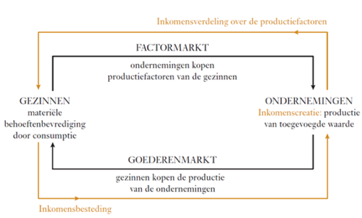
\includegraphics[width=0.65\textwidth]{Afbeeldingen/H1-Kringloop.png}
\caption{De economische kringloop, met in het zwart pijlen voor goederen en diensten, en in het grijs pijlen voor geldstromingen (in traditionele systemen gebeurt alles binnen het gezin)}
\label{fig:h1kringloop}
\end{figure}

\subsection{Comparatieve Voordelen}\label{sec:h1comp}

Beeld je nu in\footnote{Gebaseerd op het werk van David Ricardo, Brits econoom.} dat we een wereld hebben met twee landen, $R$ (rijk) en $A$ (arm). Er zijn ook twee producten, textiel en computers. $R$ beschikt over 100 eenheden arbeid en $A$ over 400 eenheden. In tabel \ref{tab:h1voordeel} staat hun arbeidsproductiviteit : hoeveel arbeid er nodig is om \'e\'en eenheid te produceren. Het is duidelijk dat $R$ rijker is, omdat diens arbeidsproductiviteit hoger is.

\begin{table}[H]
\small\centering\captionsetup{justification=centering,margin=2cm}
\begin{tabular}{l | c | c}
 & \textbf{Textiel} & \textbf{Computers} \\
\textbf{Land $R$} & 2 & 1\\
\textbf{Land $A$} & 4 & 8 \\
\end{tabular}
\caption{Arbeidsproductiviteit van landen $R$ en $A$ (de hoeveelheid arbeid die nodig is voor \'e\'en eenheid te produceren.}
\label{tab:h1voordeel}
\end{table}

Intu\"itief lijkt het beter dat land $R$ dan ook niet ruilt. Dat klopt niet. Men moet kijken naar de \entrystyled{opportuniteitskost}{opportuniteitskosten} ; de kost van, in plaats van een eenheid textiel, computers te produceren, uitgedrukt in termen van computers (tabel \ref{tab:h1oppkosten}). Of in het algemeen, de kost van een verloren gegane opportuniteit.

\begin{table}[H]
\small\centering\captionsetup{justification=centering,margin=2cm}
\begin{tabular}{l | c | c | c}
 & \textbf{Textiel} & \textbf{Computers} & \textbf{Opportuniteitskost van textiel} \\
\textbf{Land $R$} & 2 & 1 & 2 computers\\
\textbf{Land $A$} & 4 & 8 & $\frac{1}{2}$ computer \\
\end{tabular}
\caption{Arbeidsproductiviteit van landen $R$ en $A$ (de hoeveelheid arbeid die nodig is voor \'e\'en eenheid te produceren.}
\label{tab:h1oppkosten}
\end{table}

Het is duidelijk dat land $A$ een \entry{comparatief voordeel} heeft in de productie van textiel, en land $R$ een comparatief voordeel in de productie van computers.
\par Voor $A$ is het dus voordelig om zich te specialiseren in de productie van textiel en die dan te ruilen voor computers, waarin $R$ zich dan best in specialiseert. Bij onderhandeling zal $A$ zijn textiel niet kwijt willen voor minder dan $\frac{1}{2}$ computers, en zal $R$ niet meer dan 2 computers willen betalen voor een eenheid textiel. Beide gaan er dan op vooruit.
\par Economie is dus geen \entry{zero sum game} (`\term{nulsomspel}'), waarbij de ene wint wat de andere verliest.\\

\par In deze context maken we ook gebruik van \entrystyled{productiemogelijkhedencurve}{productiemogelijkhedencurven} of \entrystyled{transformatiecurve}{transformatiecurven} (zie figuur \ref{fig:h1tc}. Deze beelden productiemogelijkheden af, waarbij ervan uit wordt gegaan dat de productiemiddelen optimaal worden ingezet.

\begin{figure}[H]
\vspace{0.5cm}
\centering
\captionsetup{justification=centering,margin=2cm}
\begin{tikzpicture}
	\begin{axis}[name=left,xlabel=Landbouw, ylabel=Industrie, ymin=0,ymax=120,xmin=0,xmax=120,width=5cm, height=5cm]
		\addplot[gray, samples=100, domain=0:100]{100-(x*x)/100};
		\addplot+[draw=none,mark=none,pattern=flexible hatch, samples=100, domain=0:100, area legend, pattern color=gray!50!gray]{100-(x*x)/100} \closedcycle;
	\end{axis}
\end{tikzpicture}
\caption{Een voorbeeld van een transformatiecurve. Enkel het gearceerde gebied binnen de curve stelt productiemogelijkheden voor.}
\label{fig:h1tc}
\end{figure}

Uiteraard hebben zo'n curven negatieve hellingen, gezien de opportuniteitskosten positief zijn ; doet men meer aan landbouw, dan kan men ook minder industrieproducten produceren.
\par Bij economische groei (door demografische groei, of technologische groei) schuift de curve naar \textit{rechts}.

\subsection{Hoe Spreken Economien?}

Economen maken \textit{theorie\"en}. Omdat deze logisch moeten zijn maken ze gebruik van wiskunde. En dus is er sprake van variabelen. We categoriseren ze als stroom- en voorraadvariabelen.\\

\par Een \entry{stroomveranderlijke} heeft betrekking op een \textit{bepaalde periode}. Voorbeelden zijn het inkomen, productie, bestedingen, opbrengsten, kosten en winst.
\par Een \entry{voorraadveranderlijke} heeft betrekking op een \textit{moment}. Voorbeelden zijn de bezittingen, schulden, vermogen (bezittingen minus schulden), kapitaalstock en de geldvraag (zie later).
\par Thomas Piketty\footnote{Franse econoom die gespecialiseerd is in het thema van economische ongelijkheid vanuit een historisch en statistisch oogpunt.} heeft het vaak over de verhouding van het vermogen op het inkomen, dat in de rijke Westerse wereld ongeveer gelijk is aan zes. Hij benadrukt dat dit verschil niet te groot mag worden.\\

\par Met de variabelen stellen de economen vergelijkingen op. Stelsels van vergelijkingen vormen modellen. En deze modellen moeten overeenkomen met de werkelijkheid. Daarom toetst men ze door cijfers te verzamelen. Dit kan via observatie of experimenten (inclusief natuurlijke experimenten, zoals het uit elkaar gaan van West- en Oost-Duitsland).
\par Passen we statistiek toe op de economische gegevens, dan spreekt men van \entry{econometrie}. Hierbij is het zeer belangrijk te beseffen dat \entry{causaliteit} meer is dan \entry{correlatie} ; als twee variabelen samenhangen impliceert dit niet dat de ene variabele de andere veroorzaakt. Dit is enkel het geval als de ene de andere vooraf gaat, en er geen derde variabele is die beide variabelen bepaalt\footnote{Neem als voorbeeld Bono, die op het einde van zijn concerten in zijn handen klapt en ons vertelt dat \textit{`telkens ik klap iemand in Malaria doodgaat'}, waarna iemand in de zaal \textit{`maar stop dan toch met klappen!'} roept.}.\\

\par\noindent Economen doen ook \textit{uitspraken}. We onderscheiden positieve en normatieve uitspraken.\par
Bij een \entry{positieve uitspraak} stelt men zich de vraag, `\textit{wat is?}'. Het antwoord op zo'n vraag is juist of fout. Zo is `ja' het antwood op de vraag `\textit{kunnen we atomen splitsen?}'. In de economie helpen positieve uitspraken de samenhang tussen economische grootheden en gedragingen van economische agenten begrijpelijk te maken.\par
Bij een \entry{normatieve uitspraak} stelt men zich de vraag, `\textit{wat moet?'}. Het antwoord is niet juist of fout, er wordt nagedacht over hoe een bepaalde doelstelling het best gerealiseerd wordt. Zo zijn antwoorden op de vraag `\textit{mogen we atomen splitsen?}' normatief ; voor - en tegenstanders van kernsplitsing kunnen tal van argumenten geven om hun positie te rechtvaardigen. Uitspraken over de trade-off die men moet maken bij het kiezen tussen rechtvaardigheid en effici\"entie zijn ook normatief. \\
Economen doen best zo veel mogelijk positieve uitspraken, maar doen onvermijdelijk ook normatieve uitspraken.



